%
% Beispieldokument für TU beamer theme
%
% v1.0: 12.10.2014
% 
\documentclass{beamer}
\usetheme{TU}

\usepackage{amsmath}
\usepackage{amsfonts}
\usepackage{amssymb}
\usepackage{booktabs}
\usepackage{svg}
\def\xcolorversion{2.00}
\def\xkeyvalversion{1.8}
\usepackage{pgf}
\usepackage{tikz}
\usetikzlibrary{arrows,shapes,snakes,automata,backgrounds,petri}

\usepackage{mathtools}
\newcommand\givenbase[1][]{\:#1\lvert\:}
\let\given\givenbase
\newcommand\sgiven{\givenbase[\delimsize]}
\DeclarePairedDelimiterX\Basics[1](){\let\given\sgiven #1}
\newcommand\Average{E\Basics}

\usepackage{subfig}

\title{Explainability and Adversarial Robustness for RNNs}

\author[Alexander Hartl]{
	Alexander Hartl\inst{a} \and Maximilian Bachl\inst{a} \and \\ Joachim Fabini\inst{a} \and Tanja Zseby\inst{a}
}

\institute{%
	\inst{a}Technische Universität Wien, Vienna, Austria
}

%\session{XXXX \#}

%Kann angepasst werden, wie es beliebt. Entweder das Datum der Präsentation oder das Datum der aktuellen Präsentations-Version.
\date[\the\day.\the\month.\the\year]{\today}


\DeclareMathOperator*{\argmin}{arg\,min}

\begin{document}

% -------------
% Titlepage
% -------------
\maketitle

\section{Introduction}

\begin{frame}{Intrusion Detection Systems}
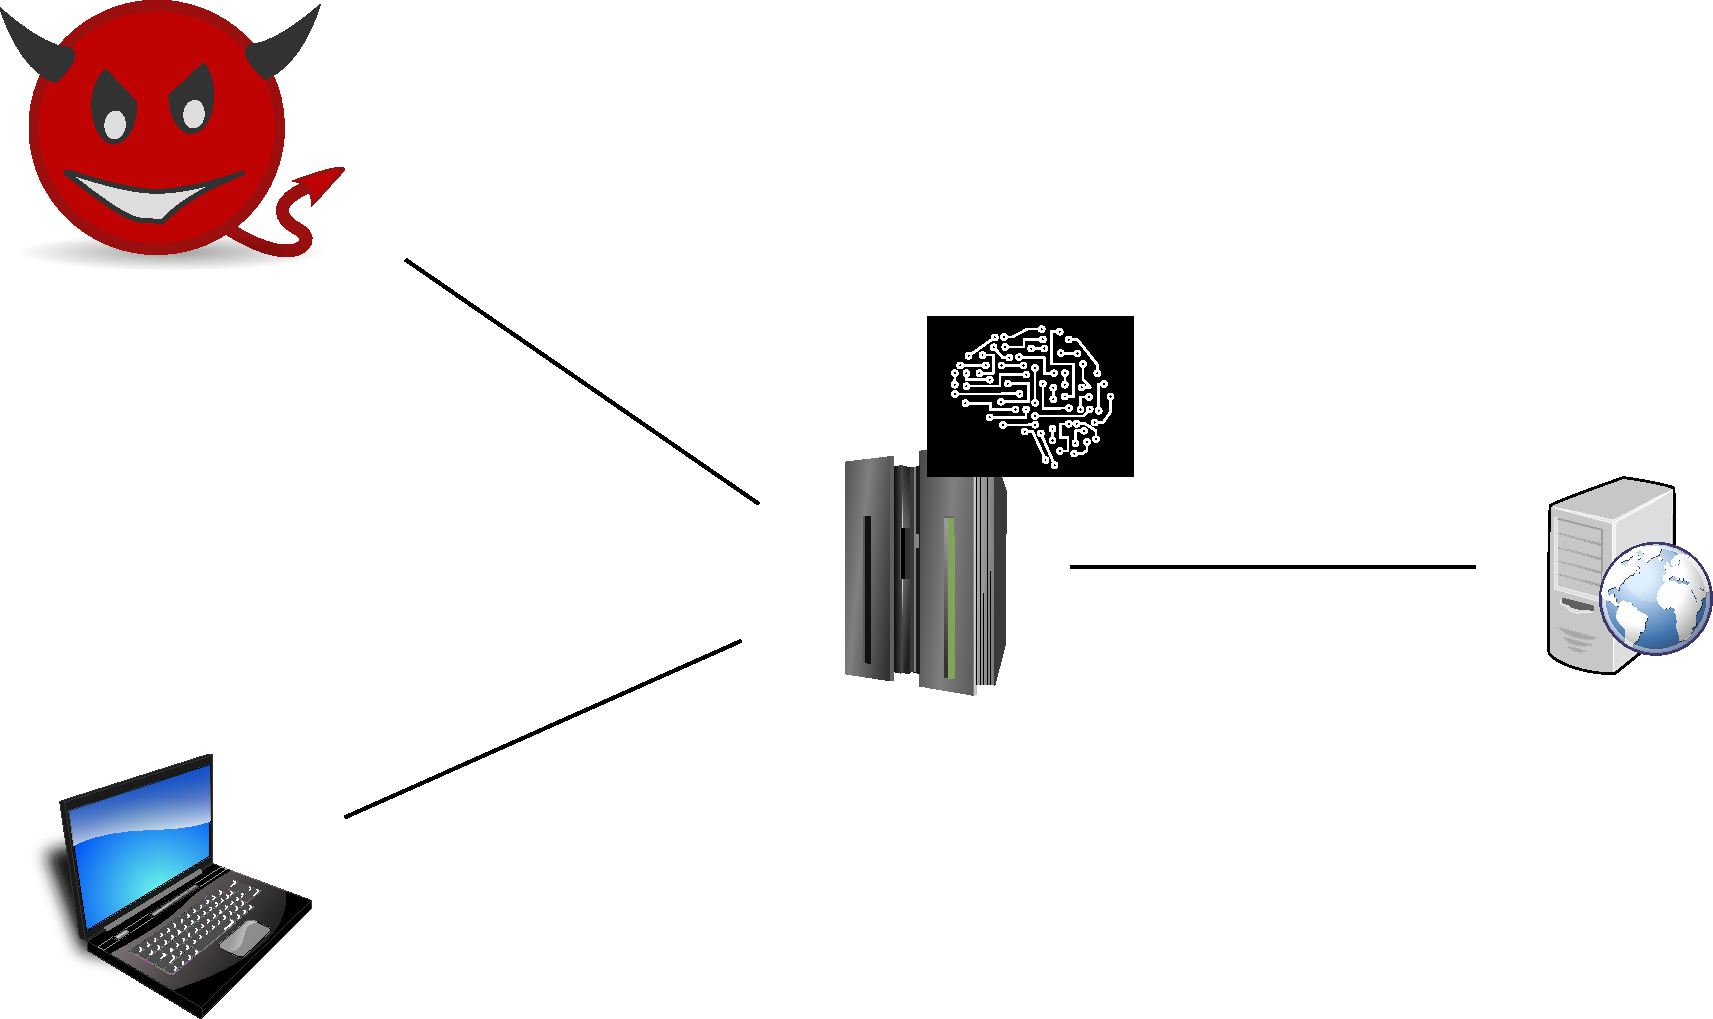
\includegraphics[width=\columnwidth]{figures/scenario.pdf}
\end{frame}

\begin{frame}{Intrusion Detection Systems}
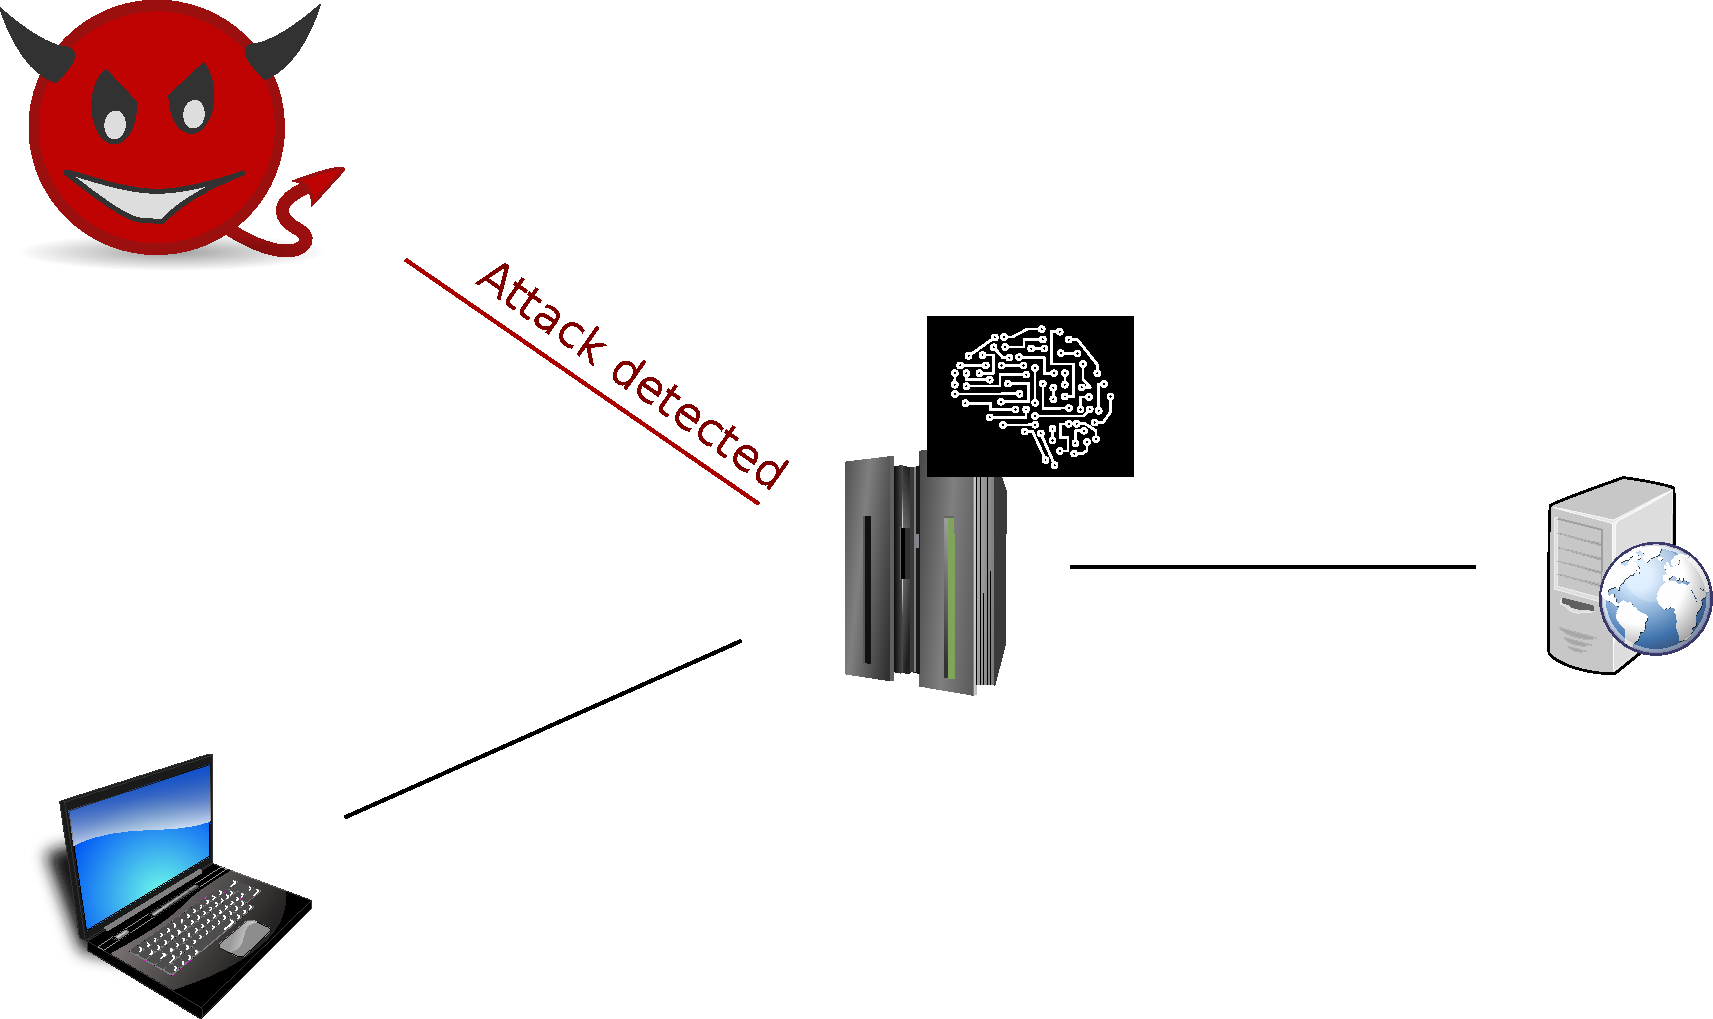
\includegraphics[width=\columnwidth]{figures/scenario2.pdf}
\end{frame}

\begin{frame}{Intrusion Detection Systems}
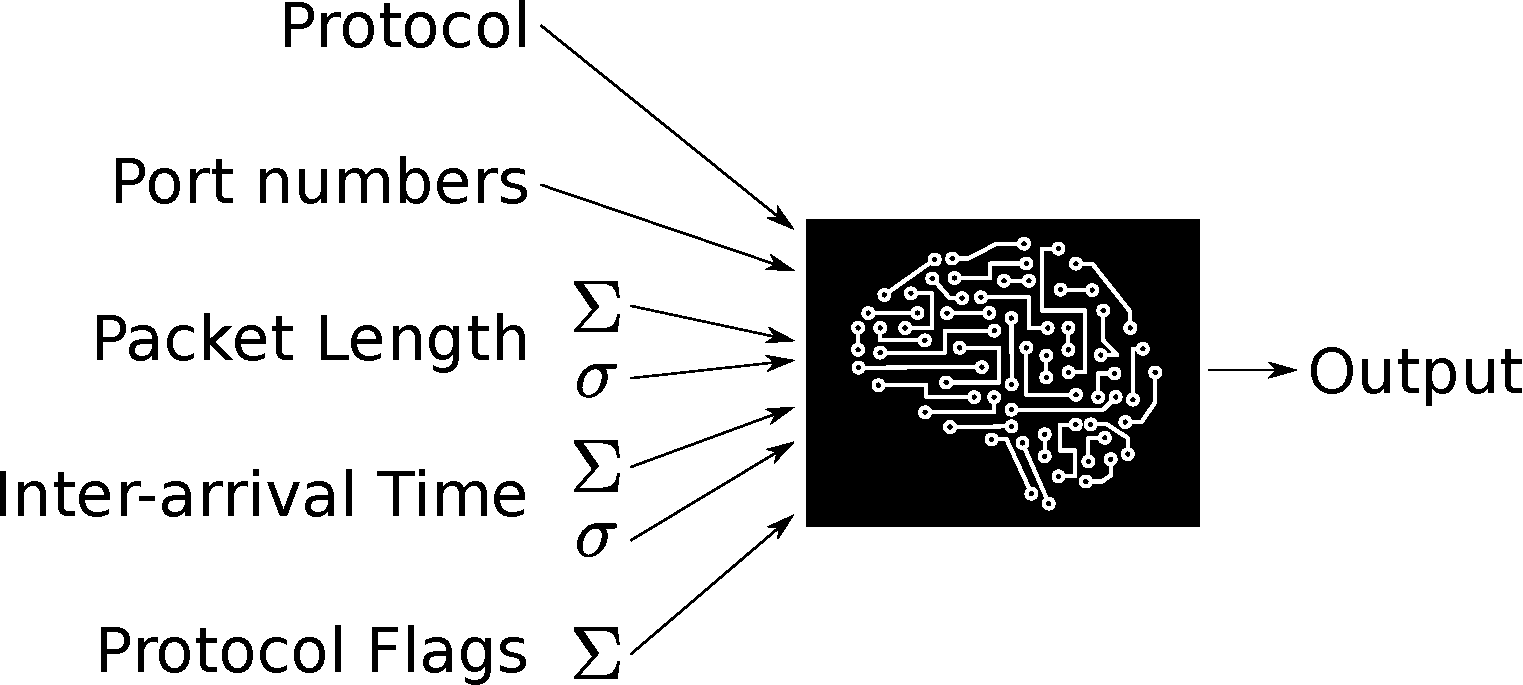
\includegraphics[width=\columnwidth]{figures/ids.pdf}
\end{frame}

\section{An RNN for Intrusion Detection}
\begin{frame}{Using a Recurrent Neural Network}
\begin{itemize}
\item Detect attacks before they are over
\item Classifier obtains all available information
\end{itemize}
\vspace{10pt}
\centering
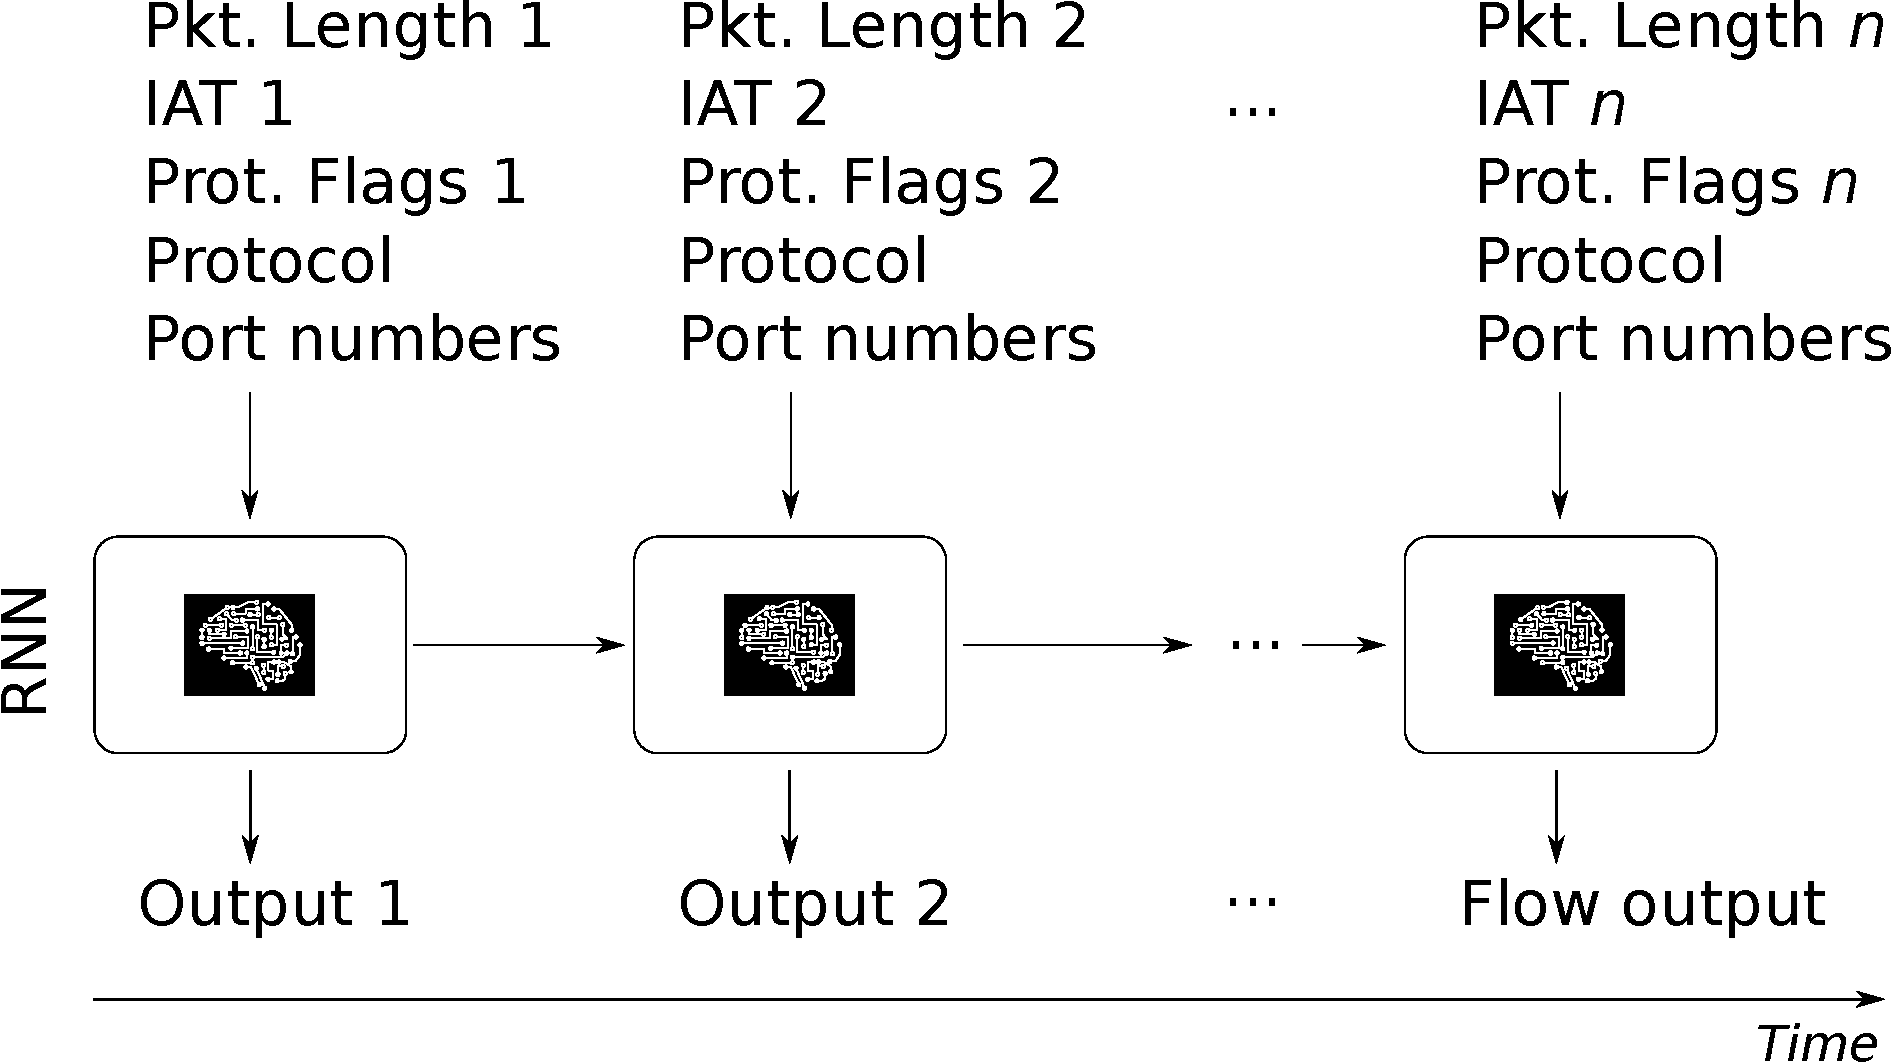
\includegraphics[width=0.8\columnwidth]{figures/rnn.pdf}
\end{frame}


\begin{frame}{Results}
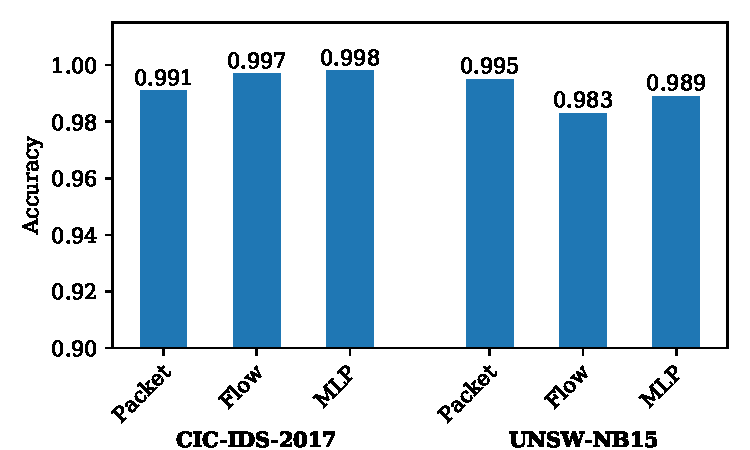
\includegraphics[width=\columnwidth]{figures/results.pdf}
\end{frame}

\begin{frame}{Results}
\vspace*{-49pt}
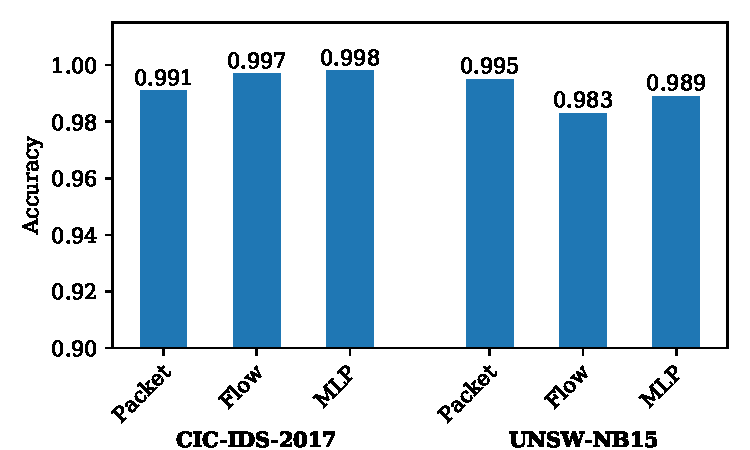
\includegraphics[width=\columnwidth]{figures/results.pdf}

\vspace*{-130pt}
\fcolorbox{black}{white}{
\begin{minipage}{0.9\textwidth}
\vspace{10pt}
\begin{itemize}
\item How does the classifier come to a decision?
\item Is it possible to trick the classifier?
\end{itemize}
\vspace{10pt}
\end{minipage}
}
\end{frame}


\section{Adversarial ML}
\begin{frame}{Adversarial Samples}
\begin{itemize}
\item Craft attack samples which are classified as benign \vspace{10pt}
\item Real-world constraints
\begin{itemize}
\item Only packets from adversary manipulable
\item Only few features can be manipulated
\item Packet length cannot decrease
\item IATs cannot decrease
\end{itemize}
\end{itemize}
\end{frame}

\begin{frame}{Finding Adversarial Samples}
\begin{itemize}
\item Carlini-Wagner {\footnotesize ($X$...orig.~sample; $Z$...logit output; $\kappa,\delta$...parameters) \hspace*{-1cm} }
\begin{equation*} \label{eq:carliniWagner}
\argmin_{\tilde X}d(X,\tilde X) + \kappa  \max(Z(\tilde X), \delta)
\end{equation*}
\item FGSM {\footnotesize ($L$...neural network loss; $\epsilon$...parameter) }
\begin{equation*}
\tilde X = X + \epsilon \, \text{sgn}( \nabla_X L(X))
\end{equation*}
\item $L_\infty$-bounded Projected Gradient Descent


\end{itemize}
\end{frame}

\begin{frame}{Finding Adversarial Samples}
\begin{figure}[h]
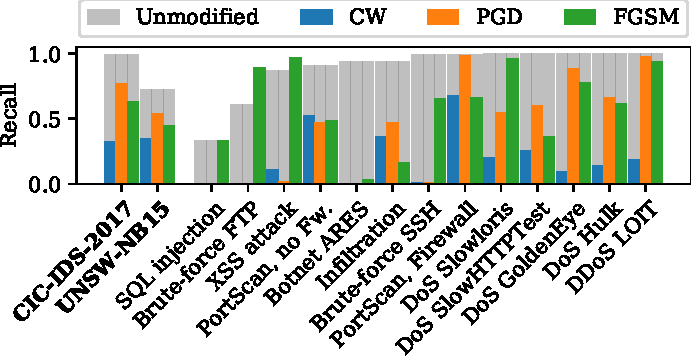
\includegraphics[width=\columnwidth]{../plots/adv_comparison/adv_comparison_17.pdf}
\end{figure}
\end{frame}

\begin{frame}{The Adversarial Robustness Score}
\begin{itemize}
\item Quantify ease of generating adversarial samples
\item Carlini-Wagner {\footnotesize ($X$...orig.~sample; $Z$...logit output; $\kappa,\delta$...parameters) \hspace*{-1cm} }
\begin{equation*} \label{eq:carliniWagner}
\argmin_{\tilde X} d(X,\tilde X) + \kappa  \max(Z(\tilde X), \delta)
\end{equation*}
\item ARS $\approx$ avg. distance of the 50\% successful adversarial samples with lowest distance
\end{itemize}
\end{frame}

\section{Explainability}
\begin{frame}{Explainability}
\begin{enumerate}
\item Feature Importance \vspace{10pt}
\item Explainability Plots \vspace{10pt}
\item Plots for Sequences
\end{enumerate}
\end{frame}

\begin{frame}{Feature Importance}
\begin{itemize}
\item Neural Network Weights
\begin{itemize}
\item simple, fast, but inaccurate
\end{itemize}
\item Input Perturbation
\begin{itemize}
\item how important is feature for accuracy
\end{itemize}
\item Feature Dropout {\footnotesize (introduced in this research) }
\begin{itemize}
\item solves problem that classifier hasn't been trained for perturbed variables
\end{itemize}
\item Mutual Information
\begin{itemize}
\item for feature \textit{sensitivity}
\end{itemize}
\end{itemize}
\vspace*{-1cm}\hspace{5cm}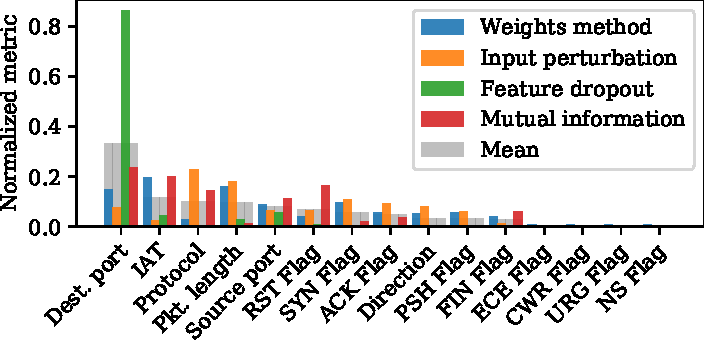
\includegraphics[width=0.6\columnwidth]{../plots/importance/feat_imp_flow_2017.pdf}
\end{frame}

\begin{frame}{Explainability Plots}

\begin{equation*}
\text{PDP}_{c,i}(w) = \mathbb E_{\boldsymbol X | C} \Big(f \left( X_1,\ldots,X_{i-1},w,X_{i+1},\ldots X_n \right) | c\Big)
\end{equation*}
\begin{figure}
\includegraphics[width=\columnwidth]{{"../../plots/plot_pdp/flows_pdp_outcomes_0_3.pickle_10_Normal"}.pdf}
\end{figure}

\end{frame}

\begin{frame}{Classifier Confidence}
How fast does RNN come to a decision?

\vspace{20pt}
\includegraphics[width=\columnwidth]{{"../plots/plot/flows_pred_plots2_outcomes_0_3.pickle_15_All_samples"}.pdf}
\end{frame}

\begin{frame}{Sequential Partial Dependence}
\begin{align*}
\text{se}&\text{qPDP}_{c,i}(t,w)= \\ &\mathbb E_{X | C} \Big(f \left(h_{t-1}( X), X_1^t,\ldots,X_{i-1}^t,w,X_{i+1}^t,\ldots X_n^t \right) | c\Big) \nonumber
\end{align*}
\centering
\includegraphics[width=0.75\columnwidth]{{"../plots/plot2_adv/flows_pred_plots2_outcomes_flows_adv_1.0_notBidirectional_outcomes_0_3.pickle_0_3.pickle_7_DoS_-_DDoS-DoS_slowloris"}.pdf}
\end{frame}

\section{Defenses}
\begin{frame}{Defenses}
\begin{itemize}
\item Omit manipulable features
\begin{itemize}
\item Either omit all packet lengths and IATs
\item or retain features in non-manipulable direction
\end{itemize}
$\rightarrow$ Surprisingly good accuracy \vspace{10pt}
\item Adversarial Training

\vspace{5pt}
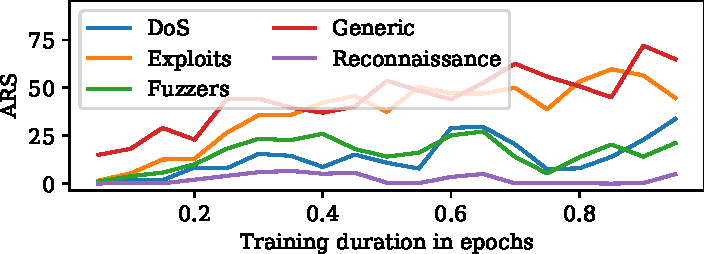
\includegraphics[width=0.7\columnwidth]{../plots/ars/ars_15.pdf}
\end{itemize}
\end{frame}

\section{Conclusions}
\begin{frame}{Conclusions}
\begin{itemize}
\item RNNs usable for IDSs
\item Adversarial ML algorithms work
\begin{itemize}
\item Defenses work, too
\item \textit{Adversarial Robustness Score} for quantifying robustness
\end{itemize}
\item Explainability
\begin{itemize}
\item Feature importance and sensitivity, dependent on purpose 
\item Visualization\\$\rightarrow$ e.g. \textit{sequential Partial Dependence Plots}
\item Find packets which are characteristic for attack
\end{itemize}
\end{itemize}
\end{frame}
% -------------
% Last page
% -------------
\makelastslide

\end{document}
